% PandaProbe Harness branded arXiv preprint for agent builders and the
% open-source community.
\documentclass[11pt,letterpaper]{article}

\usepackage[left=1.2in,right=1.2in,top=1in,bottom=1in,headheight=17pt,headsep=14pt]{geometry}
\usepackage{amsmath,amssymb}
\usepackage{newtxtext,newtxmath}
\usepackage[hyphens]{url}
\usepackage{graphicx}
\usepackage{booktabs}
\usepackage{float}
\usepackage{multirow}
\usepackage{tabularx}
\usepackage{algorithm}
\usepackage{algorithmic}
\usepackage{listings}
\usepackage{xcolor}
\usepackage{microtype}
\usepackage{enumitem}
\usepackage{xspace}
\usepackage{natbib}
\usepackage{caption}
\usepackage{titlesec}
\usepackage{tikz}
\usepackage{fancyhdr}
\usetikzlibrary{arrows.meta,positioning,fit,backgrounds,calc}
\usepackage[colorlinks=true,allcolors=blue!55!black,hypertexnames=false]{hyperref}
\hypersetup{
  pdftitle={PandaProbe Harness: Evidence-Gated Self-Healing for Reliable LLM Agents},
  pdfauthor={Sina Tayebati; PandaProbe Research Lab, Chirpz AI},
  pdfsubject={Open-source self-healing runtime envelope for LLM agents},
  pdfkeywords={LLM agents, reliability, self-healing, PandaProbe, evidence-gated validation}
}

\setcounter{secnumdepth}{2}
\setlength{\textfloatsep}{8pt plus 2pt minus 2pt}
\setlength{\floatsep}{7pt plus 2pt minus 2pt}
\setlength{\intextsep}{7pt plus 2pt minus 2pt}
\captionsetup{font=small,labelfont=bf}
\titleformat{\section}{\large\bfseries}{\thesection}{0.75em}{}
\titleformat{\subsection}{\fontsize{11}{13}\selectfont\bfseries}{\thesubsection}{0.75em}{}
\frenchspacing

\definecolor{codebg}{RGB}{246,248,250}
\lstdefinestyle{pandacode}{
  backgroundcolor=\color{codebg},
  basicstyle=\ttfamily\scriptsize,
  breaklines=true,
  columns=fullflexible,
  frame=single,
  framerule=0.25pt,
  showstringspaces=false,
  tabsize=4
}
\lstset{style=pandacode}

% Notation for the self-healing mechanism and benchmark study.
\newcommand{\ind}{\mathbf{1}}
\newcommand{\Rset}{\mathcal{R}}
\newcommand{\evalfn}{\mathcal{E}}
\newcommand{\mvec}{\mathbf{m}}
\newcommand{\Heal}{\mathcal{H}}
\newcommand{\Breach}{\mathfrak{B}}
\newcommand{\dpromote}{\delta_{\mathrm{prom}}}
\newcommand{\dregress}{\delta_{\mathrm{reg}}}
\newcommand{\passk}{\mathrm{pass}^{k}}
\newcommand{\passone}{\mathrm{pass@}1}
\newcommand{\TBD}{--}
\newcommand{\topk}{\textsc{top-}k}
\newcommand{\Harness}{\textsc{PandaProbe Harness}\xspace}
\newcommand{\PandaProbe}{\textsc{PandaProbe}\xspace}

% --- Branding: logo, running head, and the ruled title block --------------------
% Logo height is a multiple of the surrounding font's cap height (queried from the
% font metrics), so it tracks any font-size change with no per-use tuning. A factor
% of 1.0 is exactly cap height, which reads short because the PNG carries internal
% padding, so 1.45 sits the visible mark on the capitals beside it.
\newcommand{\pplogo}{%
  \raisebox{-0.16\height}{%
    
\includegraphics[height=\dimexpr1.45\fontcharht\font`P\relax]{logo/android-chrome-512x512}}%
}
\newcommand{\shorttitle}{PandaProbe Harness: Evidence-Gated Self-Healing}
\newcommand{\reportkind}{Technical Report}

\pagestyle{fancy}
\fancyhf{}
\fancyhead[C]{\small\pplogo\hspace{0.32em}\shorttitle}
\fancyhead[R]{\small\scshape\reportkind}
\fancyfoot[C]{\small\thepage}
\renewcommand{\headrulewidth}{0.5pt}
\renewcommand{\footrulewidth}{0pt}
% v0.7 tiered trace trigger + trajectory gate
\newcommand{\Mset}{\mathcal{M}}
\newcommand{\Gate}{\mathcal{G}}
\newcommand{\Wspace}{\mathcal{W}}
\newcommand{\gwin}{w}
\newcommand{\gtarget}{\theta}
\newcommand{\ggain}{\gamma_{\mathrm{gain}}}
\newcommand{\gdrop}{\delta_{\mathrm{drop}}}
\newcommand{\outcome}{m_{\mathrm{out}}}
\newcommand{\idx}{\iota}

\title{PandaProbe Harness: Evidence-Gated Self-Healing for Reliable LLM Agents}
\author{
  Sina Tayebati\\
  \small PandaProbe Research Lab, Chirpz AI\\
  \small \href{https://github.com/chirpz-ai/pandaprobe-harness}{github.com/chirpz-ai/pandaprobe-harness}
}
% TODO(author): confirm exact author spelling, affiliation, email, ORCID, and co-authors.
\date{}

\begin{document}

% Ruled title block: heavy rule, small-caps title with the logo, heavy rule,
% then the report kind and the author line.
\begin{center}
  \rule{\textwidth}{1.1pt}\\[0.62em]
  {\LARGE\scshape \pplogo\hspace{0.36em} PandaProbe Harness:\\[0.28em]
   Evidence-Gated Self-Healing for Reliable LLM Agents\par}
  \vspace{0.58em}
  \rule{\textwidth}{1.1pt}\\[0.85em]
  {\normalsize\scshape \reportkind\ of the PandaProbe Harness}\\[1.0em]
  {\normalsize Sina Tayebati}\\[0.25em]
  {\small PandaProbe Research Lab, Chirpz AI}\\[0.15em]
  {\small\href{https://github.com/chirpz-ai/pandaprobe-harness}{github.com/chirpz-ai/pandaprobe-harness}}
\end{center}
\thispagestyle{plain}
\vspace{0.6em}

\begin{abstract}
\noindent
Large language model (LLM) agents that are \emph{capable} on a task are not necessarily
\emph{reliable} on it: the same agent, run repeatedly, frequently succeeds on some trials and
fails on others, and quality tends to drift over long horizons. Peak-performance metrics such
as $\passone$ hide this variance, whereas the stricter reliability metric $\passk$, the
fraction of tasks solved on \emph{all} $k$ independent trials, exposes it. We present
\Harness, an open-source runtime envelope developed and maintained by the PandaProbe research lab
that wraps an arbitrary developer-owned LLM agent loop and, with no human in the loop,
(i) \emph{detects} quality degradations from PandaProbe's trace-level evaluation layer,
(ii) posts structured diagnostic notices to an inspectable workspace, (iii) assigns each notice
to a separate package-owned repair agent that authors corrective operating \emph{rules},
and (iv) admits each rule only after an empirical \emph{evidence gate}: replay of the captured failure or a forward
trial over subsequent live sessions, with a regression guard for past wins. Validated rules reach
the task agent only by \emph{pull}: its prompt carries one constant capability sentence and four
read-only tools, and no rule text is ever injected. Detection is
deliberately structured, because a gate is only as good as the signal that invokes it. \Harness
scores every \emph{trace} of a session with cheap always-on metrics and judges the
\emph{trajectory} they trace out, so an unfinished task is not mistaken for a failing one; it
escalates to costly step-level diagnosis only once a \emph{trajectory gate} reports a stall or a
regression; a per-turn barrier makes each proposed rule visible \emph{within} the session that
motivated it; and an optional outcome verifier lets the gate decide on ground truth rather than a
proxy. We formalize the loop as an evidence-gated operator on the agent's policy-inducing context
and cast rule validation as paired empirical improvement testing with a multi-metric
non-regression constraint. We evaluate four open-weight task models on the three $\tau^2$-bench
domains and a 10-task Terminal-Bench sample, with one seed and four trials per task. Across 13
completed baseline--Harness pairs, strict $\passone$ improves in three and $\passk$ in seven;
the paired $\passone$ intervals all include zero. Validation is dominated by forward trials,
and the additional repair-model spend is substantial. These results characterize the current
single-seed configuration rather than establishing a uniform reliability gain.
\end{abstract}

\section{Introduction}
\label{sec:intro}

Progress on LLM agents is usually reported as \emph{capability}: can the agent, at its best,
solve the task? Deployment demands \emph{reliability}: does it solve the task \emph{every}
time it is asked? These are different properties. Modern agents are stochastic, and some
frontier models do not expose temperature control, so repeated runs of the same agent on the
same task yield different outcomes. A metric such as $\passone$ rewards a successful first
draw; $\passk$ asks whether \emph{all} $k$ independent trials pass. Closing this
\emph{reliability gap} is the problem we attack.

A natural idea is to let the agent correct itself. Existing methods reflect on failed attempts
and retry \citep{shinn2023reflexion,madaan2023selfrefine,gou2024critic}. Such open-loop
self-correction has two limitations. First, it is \emph{unvalidated}: a plausible-sounding
reflection is trusted immediately, even when it degrades behavior. Second, it is commonly
\emph{within-episode}: the lesson does not reliably survive to the next task. Reliability is a
cross-episode property, so a mechanism that neither persists nor verifies corrections is poorly
matched to it.

\Harness closes the loop. It wraps an arbitrary agent as a non-blocking runtime envelope and
runs four stages across episodes: \textbf{Detect}, \textbf{Notice}, \textbf{Heal}, and
\textbf{Validate} (Figure~\ref{fig:overview}). PandaProbe scores completed sessions. Diagnostic
notices are persisted in a filesystem workspace consumed by a package-owned repair agent; the
developer's task agent never receives diagnostic or administrative capabilities. The repair agent
authors a corrective rule, but that rule enters as a provisional candidate and becomes active only
after replay or forward-trial evidence. Later task turns may \emph{read} what was learned through
four read-only tools, while a replayable eval-set protects previous wins against regression.

PandaProbe Harness is a Python package developed and maintained by PandaProbe, a research lab at
Chirpz AI building open infrastructure for reliable agent systems. Task evaluation reaches the
PandaProbe platform through its public CLI; repair-agent model calls use the PandaProbe SDK's
official LiteLLM wrapper and tracing integration. Project resources are available at:
\begin{itemize}[leftmargin=*,itemsep=0pt,topsep=2pt]
\item \textbf{GitHub repository:}\\[-1pt]
  \href{https://github.com/chirpz-ai/pandaprobe-harness}{\nolinkurl{https://github.com/chirpz-ai/}}\\[-1pt]
  \href{https://github.com/chirpz-ai/pandaprobe-harness}{\nolinkurl{pandaprobe-harness}}
\item \textbf{Documentation:}\\[-1pt]
  \url{https://docs.pandaprobe.com/harness}
\end{itemize}

\paragraph{Contributions.}
\begin{enumerate}[leftmargin=*,itemsep=2pt]
\item \textbf{Self-healing as a drop-in reliability layer.} PandaProbe Harness wraps raw loops
and common agent frameworks without weight updates, transcript mutation, or a human healing loop.
Its workspace and journal make adaptation inspectable and reversible.
\item \textbf{An evidence gate for self-improvement.} We formalize replay-based paired
improvement with a multi-metric non-regression constraint, a forward-trial test on breach
proportions, and a corpus-level regression guard (\S\ref{sec:validate}--\S\ref{sec:regression}).
\item \textbf{A reliability-first evaluation protocol.} We compare baseline and Harness arms
using $\passone$, $\passk$, paired score statistics, validation-path telemetry, and explicit
overhead accounting on $\tau^2$-bench and a Terminal-Bench sample.
\item \textbf{A capability boundary between doing and diagnosing.} Rule authoring is moved out of the
task agent entirely: it keeps four read-only tools and a constant preamble, a package-owned repair
agent holds the nine-operation diagnostic surface, and neither can promote or retire a rule.
\item \textbf{An open implementation surface.} The released package provides a small facade,
six framework adapters, four read-only task tools, a restricted repair-agent tool surface,
offline examples, operator CLIs, and a reproducible benchmark project for community extension.
\end{enumerate}

\section{Background and Related Work}
\label{sec:related}

\paragraph{Self-refinement and reflection.}
Iterative self-refinement can improve an answer \citep{madaan2023selfrefine}. Reflection on failed
episodes \citep{shinn2023reflexion} and tool-assisted critique \citep{gou2024critic} provide
related feedback loops. They largely adopt corrections without an external test. PandaProbe
Harness persists corrections across episodes and admits them only after measured evidence.

\paragraph{Verification and self-consistency.}
Sampling reasoning paths and voting \citep{wang2023selfconsistency}, or scoring outputs with an
LLM judge \citep{zheng2023judging}, improves inference-time selection but does not change the
agent's standing operating context. We apply outcome-based verification to durable rules rather
than individual answers.

\paragraph{Agent memory and experiential learning.}
Long-lived agent memory \citep{packer2023memgpt,park2023generative}, skill libraries
\citep{wang2023voyager}, and retrieval-augmented generation \citep{lewis2020rag} let systems
reuse experience. Harness rules are a compact, human-readable memory with an admission-control
step: candidates are evidence-gated and may be retired.

\paragraph{Steering, guardrails, and observability.}
Rule-based steering \citep{bai2022constitutional} and runtime guardrails constrain or monitor
behavior. Here rules are self-authored in response to PandaProbe session signals, and monitoring
is closed back into the agent's policy-inducing context. The deterministic Harness owns storage,
retrieval, validation, and regression; the model owns only diagnosis and proposal.

\paragraph{Reliability metrics and benchmarks.}
We measure reliability with $\passk$ on Terminal-Bench and $\tau^2$-bench
\citep{merrill2026terminal,barres2025tau}. Paired task bootstrap intervals
\citep{efron1993bootstrap} quantify uncertainty in score differences.

\section{PandaProbe Harness}
\label{sec:harness}

We first fix notation (Table~\ref{tab:notation}), then define the four stages and the objects
they operate on. Predicates, constants, and defaults below match the open-source implementation.

\begin{table}[t]
\centering
\caption{Notation used throughout the paper.}
\label{tab:notation}
\begin{tabularx}{0.85\textwidth}{@{}lX@{}}
\toprule
Symbol & Meaning \\
\midrule
$\pi$ & fixed agent policy being wrapped \\
$s=(x_1,\ldots,x_T)$ & one task-trial session and its traces \\
$x_i$ & the $i$-th trace (one agent turn) \\
$\evalfn$ & PandaProbe trace-level evaluator \\
$m_j(x)$ & metric $j$ on trace $x$; $\varnothing$ if pending \\
$\Mset_\ell$ & metric set of tier $\ell\in\{0,1,2,3\}$ \\
$\Gate$ & trajectory gate (stall / regression) \\
$\gwin,\gtarget$ & gate window, target (default $5$, $0.5$) \\
$\ggain,\gdrop$ & gain / drop margins ($0.02$, $0.15$) \\
$\tau_j$ & absolute threshold, tiers $0,2$ (default $0.5$) \\
$\outcome$ & optional outcome-verifier score (tier $0$) \\
$\Rset$ & active $\cup$ candidate rule set, by scope \\
$c_0$ & constant capability preamble (no rule text) \\
$\idx$ & generated rule-reference index (read on demand) \\
$\Heal$ & self-heal operator \\
$\Breach_t$ & conditions observed at turn $t$ \\
$\dpromote,\dregress$ & margins (default $0.05$) \\
$p_0,\hat p$ & baseline/trial flagged-session rates \\
\bottomrule
\end{tabularx}
\end{table}

\begin{figure}[t]
\centering
\resizebox{\textwidth}{!}{% Figure 1: PandaProbe Harness architecture and repair loop.
%
% Stage layout is a crossing-free rectangular circuit: Detect (top-left) ->
% Notice (top-right) -> Repair (bottom-right) -> Validate (bottom-left) ->
% Detect. Store order under the stages is chosen so each stage's dotted write
% arrow runs (near-)vertically instead of crossing a sibling's.

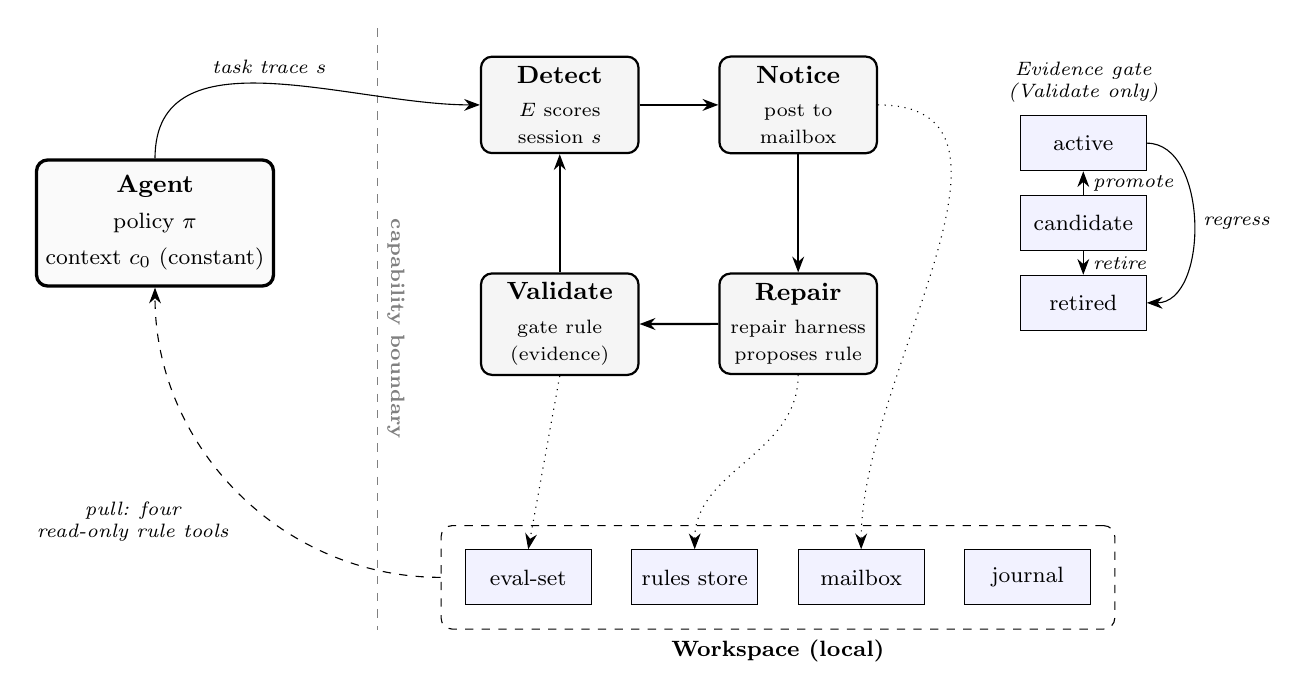
\begin{tikzpicture}[
    font=\small,
    >={Stealth[length=2mm]},
    stage/.style={draw, rounded corners, align=center, minimum width=20mm,
                  minimum height=9mm, fill=black!4, thick},
    store/.style={draw, align=center, minimum width=16mm, minimum height=7mm,
                  fill=blue!5, font=\footnotesize},
    agent/.style={draw, rounded corners, align=center, minimum width=26mm,
                  minimum height=16mm, fill=black!2, very thick},
    lbl/.style={font=\scriptsize\itshape, align=center},
    node distance=9mm and 12mm,
]

% --- Agent side (left) ---
\node[agent] (agent) {\textbf{Agent}\\[2pt]\footnotesize policy $\pi$\\[2pt]
                      \footnotesize context $c_0$ (constant)};

% --- Four stages of the loop (right), arranged as a cycle ---
\node[stage, right=26mm of agent, yshift=15mm] (detect)  {\textbf{Detect}\\[1pt]\scriptsize $E$ scores\\[-1pt]\scriptsize session $s$};
\node[stage, right=10mm of detect]             (notice)  {\textbf{Notice}\\[1pt]\scriptsize post to\\[-1pt]\scriptsize mailbox};
\node[stage, below=15mm of notice]             (repair)  {\textbf{Repair}\\[1pt]\scriptsize repair harness\\[-1pt]\scriptsize proposes rule};
\node[stage, below=15mm of detect]             (validate){\textbf{Validate}\\[1pt]\scriptsize gate rule\\[-1pt]\scriptsize (evidence)};

% Cyclic arrows: Detect -> Notice -> Repair -> Validate -> Detect.
% A rectangular circuit, so no two stage arrows cross.
\draw[->, thick] (detect)   -- (notice);
\draw[->, thick] (notice)   -- (repair);
\draw[->, thick] (repair)   -- (validate);
\draw[->, thick] (validate) -- (detect);

% --- Workspace substrate (bottom) ---
% Ordered eval-set, rules store, mailbox, journal so that Validate (bottom-left)
% and Repair (bottom-right) write straight down and Notice's arrow can pass
% clear of the Repair node on the right.
\node[store, below=22mm of validate, xshift=-4mm] (evalset) {eval-set};
\node[store, right=5mm of evalset]                (rules)   {rules store};
\node[store, right=5mm of rules]                  (mailbox) {mailbox};
\node[store, right=5mm of mailbox]                (journal) {journal};
\begin{scope}[on background layer]
  \node[draw, dashed, rounded corners, fit=(evalset)(journal),
        inner sep=3mm, label={[font=\footnotesize\bfseries]below:Workspace (local)}] (ws) {};
\end{scope}

% --- Evidence gate state machine (candidate -> active | retired) ---
% Anchored between the two stage rows rather than beside one stage: only
% Validate drives these transitions, so sitting flush against Repair would
% wrongly suggest the repair agent can promote or retire.
\node[store, right=18mm of notice, yshift=-15mm] (cand)  {candidate};
\node[store, above=3mm of cand]                  (act)   {active};
\node[store, below=3mm of cand]                  (ret)   {retired};
\draw[->] (cand) -- node[lbl,right]{promote} (act);
\draw[->] (cand) -- node[lbl,right]{retire}  (ret);
\draw[->] (act.east) to[out=0,in=0] node[lbl,right]{regress} (ret.east);
\node[lbl, above=1pt of act] {Evidence gate\\\scriptsize(Validate only)};

% --- Capability boundary (dashed vertical line between task and harness) ---
\coordinate (btop) at ($(agent.north east)!0.5!(detect.north west) + (0,10mm)$);
\coordinate (bbot) at (btop |- ws.south);
\draw[dashed, gray] (btop) -- (bbot)
      node[midway, sloped, above, font=\scriptsize\bfseries, gray] {capability boundary};

% The task agent pulls rules from the workspace; nothing is pushed to it.
\draw[->, dashed] (ws.west) to[out=180,in=270] node[lbl,below left]{pull: four\\read-only rule tools} (agent.south);

% The loop's stages read/write the workspace (harness side only).
\draw[->, dotted] (validate.south) -- (evalset.north);
\draw[->, dotted] (repair.south) to[out=270,in=90] (rules.north);
\draw[->, dotted] (notice.east) to[out=0,in=90] (mailbox.north);

% Detect reads the agent's session (the only arrow crossing toward the harness)
\draw[->] (agent.north) to[out=90,in=180] node[lbl,above]{task trace $s$} (detect.west);

\end{tikzpicture}
}
\caption{\textbf{The PandaProbe Harness self-heal loop.} After each \emph{turn}, PandaProbe scores
the turn's new traces on the always-on tier-1 metrics and the trajectory gate $\Gate$ judges the
shape of the series; a stall or regression escalates to tier-2 step-level diagnosis on the latest
trace (\textbf{Detect}). The finding becomes a notice in the workspace (\textbf{Notice}); a
separate package-owned repair agent claims it, inspects only assigned evidence, searches existing
rules, and may write a candidate (\textbf{Heal}). The candidate is promoted only after replay or a
forward trial and is retired if it regresses (\textbf{Validate}). A per-turn barrier waits for
evaluation and bounded repair before the next task turn. The capability boundary leaves the task
agent with a constant capability sentence and four read-only rule tools it may pull from --- never
mailbox, rule-write, or lifecycle access.}
\label{fig:overview}
\end{figure}

\subsection{Agent, session, and trace-level evaluation}
\label{sec:detect}

An agent is a policy $\pi$ producing actions over a session $s$. A session is not atomic: it is a
sequence of \emph{traces} $s=(x_1,\ldots,x_T)$, one per agent turn, and \Harness builds its trigger
on that decomposition. PandaProbe's evaluation layer implements a trace-level evaluator $\evalfn$
that scores an individual trace on a requested metric set, returning values in $[0,1]$ with higher
better, or \emph{pending} ($\varnothing$) when the service is transiently unavailable. The Harness
reaches PandaProbe evaluation through a CLI/JSON seam that is easy to exercise against a stand-in.
Failures degrade to pending scores and never raise into the host loop.

\paragraph{Why not a single session score.}
The natural design scores each completed session with one or two aggregate quality metrics and
alerts below a threshold. PandaProbe exposes exactly such composites: a session risk score built by
trajectory-risk aggregation over a session's most at-risk traces \citep{tayebati2026tracer}, and a
session stability score built by situational uncertainty propagation \citep{zhao2024saup}. Both are
deliberately worst-case aggregations, which is the right property for \emph{ranking} sessions post
hoc and the wrong one for gating a live loop: on long-horizon agent tasks they concentrate near the
bottom of their range for essentially every session, so a fixed-threshold trigger over them fires
almost always. The deeper issue is conceptual. A low score on a partially completed task is not
evidence of malfunction, it is the correct reading of an unfinished task, so a useful trigger has to
distinguish \emph{not yet} from \emph{not going to be}. That distinction lives in the series, not in
any single value.

\paragraph{The metric ladder.}
\Harness therefore partitions metrics into tiers by cost and role and spends the expensive ones only
where a cheaper tier already found something:
\begin{itemize}[leftmargin=*,itemsep=1pt]
\item $\Mset_1$ (\emph{progress}, always on): task completion and coherence, scored on
\emph{every} new trace of every turn. Both are cheap, and coherence is embedding-based rather
than model-judged, so the always-on rung is also the least expensive one.
\item $\Mset_2$ (\emph{step diagnosis}): tool correctness and argument correctness, on the
latest trace only and only once $\Mset_1$ has flagged the trajectory. This localizes a failure
to a step.
\item $\Mset_3$ (\emph{explanatory}, opt-in): plan adherence, plan quality, and step
efficiency, run only to enrich a confirmed $\Mset_2$ finding, never a trigger of their own.
\item $\Mset_0$ (\emph{outcome}): one score from an optional developer verifier
(\S\ref{sec:verifier}).
\end{itemize}

\paragraph{The trajectory gate.}
A tier-1 metric is judged on the \emph{shape} of its per-trace series, not its level. For metric $j$
the gate $\Gate$ keeps a running peak $\mathrm{pk}_j$ and a counter $z_j$ of traces since the last
real gain. A value clearing the peak by $\ggain$ is a gain: it raises the peak and resets $z_j$.
Otherwise $z_j$ increments and two conditions are tested,
\begin{align}
\mathrm{stall}_j(x_i)&=\ind\!\left[z_j\ge\gwin\ \wedge\ \mathrm{pk}_j<\gtarget\right],
  \label{eq:stall}\\
\mathrm{regr}_j(x_i) &=\ind\!\left[m_j(x_i)<\mathrm{pk}_j-\gdrop\right].
  \label{eq:regr}
\end{align}
% source: evaluation/trajectory.py TrajectoryGate._decide
Three properties follow, and each is deliberate. A session that keeps improving \textbf{never}
fires, however low it starts. The stall test compares the \emph{peak} against $\gtarget$ rather than
the current value, so a session that has genuinely reached its target may plateau freely. Progress
is measured against the peak, so oscillation around a plateau does not read as progress. The gate
fires once and then reopens a fresh window, so one stall yields one escalation rather than one per
subsequent trace. Defaults: $\gwin{=}5$, $\gtarget{=}0.5$, $\ggain{=}0.02$, $\gdrop{=}0.15$;
\texttt{HARNESS\_GATE\_WINDOW} is the primary knob, since the right window depends on task horizon.

\paragraph{Absolute breaches, and where they apply.}
For metric $j$ with threshold $\tau_j$ the point breach is
\begin{equation}
  b_j(x)=\ind\!\left[m_j(x)\ne\varnothing\ \wedge\ m_j(x)<\tau_j\right],
  \label{eq:breach}
  % source: evaluation/metrics.py MetricScore.breached
\end{equation}
strict, with a missing score never a breach. This indicator is consulted only for tiers $\{0,2\}$:
\begin{equation}
  \mathrm{breach}_j(x)=b_j(x)\ \wedge\ \mathrm{tier}(j)\in\{0,2\}.
  \label{eq:absbreach}
  % source: evaluation/metrics.py ABSOLUTE_BREACH_TIERS = {0, 2}
\end{equation}
A tier-1 floor is deliberately \emph{not} a fault, since its verdict is
Eqs.~\eqref{eq:stall}--\eqref{eq:regr}, and tier 3 never breaches because it runs only to explain a
finding another tier already made.

\paragraph{Escalation and severity.}
Tier 1 runs on every new trace; if nothing stalls or regresses the turn is clean and nothing further
is spent. Otherwise tier 2 runs on the last trace $x_T$, and severity depends on whether it
corroborates the trajectory finding:
\begin{equation}
\mathrm{sev}=
\begin{cases}
\texttt{breach}&\exists j\in\Mset_2\cup\Mset_0:\mathrm{breach}_j(x_T),\\
\texttt{trend} &\text{otherwise (advisory).}
\end{cases}
\label{eq:sev}
% source: hook/core.py _severity; _persist_notice captures only on "breach"
\end{equation}
Only a \texttt{breach}, a trajectory finding that step-level metrics confirm, is captured as a
replayable case for the gate (\S\ref{sec:validate}); an uncorroborated wobble is still reported
but is not treated as promotable training signal. Fired conditions become
\emph{condition}:\emph{metric} signatures, e.g.\ a stall on task completion or a breach on tool
correctness, used downstream for de-duplication, tagging, and case matching.

\paragraph{Cost.}
The ladder is the primary cost control, not an optimization detail. Tier 1 covers a turn's new
traces in a \emph{single} batched PandaProbe run; tier 2 touches one trace and only after a gate
fire; tier 3 is off by default. Because each model-judged metric reads a whole trace, cost scales
with metrics actually run, which is what makes always-on trajectory monitoring affordable.

\subsection{The per-turn barrier}
\label{sec:barrier}

Detection is worthless if the correction arrives after the task is over. \Harness therefore exposes
a per-turn \emph{barrier}: \texttt{settle(session\_id)}, also reachable as a \texttt{settle=True}
flag on the turn scope, which waits until the turn's evaluation has resolved, its
report has been handled, any case captured, any notice posted, and one bounded repair
attempt has completed or timed out. The \emph{next} turn therefore observes any candidate this
turn produced. It runs on its own budget
(\texttt{barrier\_timeout\_s}, default 180\,s), separate from the best-effort drain joins used
elsewhere. Evaluation may continue detached on barrier expiry; a timed-out repair is cancelled,
journaled, and leaves its notice recoverable. Neither failure path fails the developer's task.
Replay validation remains detached because the task may hold a non-reentrant environment lock.

The barrier is also a precondition for the gate to function at all. Score history is keyed per
session, so a host that synchronizes once per \emph{task} contributes one sample per series, the
stall window of Eq.~\eqref{eq:stall} can never close, and the trajectory machinery is silently
inert. This is an easy integration error to make and a hard one to notice, because the loop appears
to run and simply never fires: delimit \emph{turns}, not tasks.

\subsection{The outcome verifier}
\label{sec:verifier}

Every metric above is a judged proxy. When a developer already knows what success means, a golden
dataset, a benchmark grader, a database assertion, \Harness accepts that oracle directly as a
\texttt{verifier} argument to the factory, taking the session id and the turn's end-state:
\begin{equation}
  \outcome(s)\in[0,1]\cup\{\varnothing\}.
  \label{eq:verifier}
  % source: hook/tiers.py VerifierFn, run_verifier
\end{equation}
Abstention is a first-class answer: a grader that can only score a \emph{finished} task returns
$\varnothing$ on intermediate turns. A verdict enters as a tier-0 metric, so unlike tier 1 it
\emph{does} breach on absolute value against a strict $\tau_{\mathrm{out}}{=}0.9$. Exceptions are
caught and the turn proceeds without an outcome score, so a faulty oracle cannot break the host
loop. Because it depends only on the end-state it is evaluated concurrently with the ladder.

The verifier matters most at the gate, where a ground-truth outcome is strictly better evidence
than a proxy (\S\ref{sec:validate}). One caution belongs in the mechanism rather than a footnote,
because it is the same failure mode that motivated the trajectory gate: a \emph{binary} pass/fail
oracle on hard tasks is almost never positive, and a signal that is almost never positive
discriminates nothing. Prefer continuous partial credit. Our own AppWorld integration is a concrete
case: over a 40-trial measurement the benchmark's binary success flag was positive on 1 trial while
the mean fraction of its unit tests passed was $0.70$, so the flag would have declared failure on
$97.5\%$ of sessions where the continuous score separates near-misses from genuine breakdowns. We
therefore wire the pass fraction, not the flag.
% source: benchmarks/src/pandabench/runners/appworld.py outcome_for

\subsection{Read-only rules from the harness workspace}
\label{sec:retrieval}

Learned rules must reach the agent somehow, and inlining them into the system prompt does not
survive a growing corpus. Two costs grow with the rule set: tokens, and \emph{attention}. In a
measured run of a build that inlined the whole corpus alongside a large self-diagnostic tool
surface, the agent reoriented toward operating the Harness rather than doing the task, and most of
the rules it authored concerned its own diagnostic protocol rather than the work. The token cost is
equally concrete. Comparing that build against the current one on the same AppWorld task set and
model (228 task-trials each), we group trials by how many rules were active when they ran: with at
most two active rules the inlining build read $11.6$k input tokens per turn, and with more than two it
read $46.5$k, a $4.0\times$ inflation driven purely by rules the agent had not asked for and whose
peak trial reached $148$k. Under the pull model the same contrast is $5.4$k versus $5.3$k --- flat,
because what the prompt carries no longer depends on what the corpus holds. Growth in what the agent
has learned must not become growth in what it must read every turn.

\Harness therefore \emph{pushes nothing}. The task preamble is a constant,
\begin{equation}
  c(\Rset,s,q)=c_0,
  \label{eq:context}
  % source: hook/context.py compose_system_preamble (task_hint deleted, *_args discarded)
\end{equation}
one sentence stating that learned rules exist and naming the four read-only tools that reach them.
It is independent of $\Rset$, of the session $s$, and of any task hint $q$: constructing it performs
no read, search, or ranking, so no eval-derived text can enter a task prompt automatically.
Retired rules are never readable; a candidate written after turn $t$ is discoverable on turn $t{+}1$
because the barrier (\S\ref{sec:barrier}) lands it before the turn begins, not because anything
inserts it. No mailbox banner, notice count, scope index, or repair instruction enters task context.

The agent \emph{pulls} when it judges prior rules relevant, through exactly four operations: list
(the generated guide $\idx$ plus a live scope index with counts), read (one scope file), search, and
status (one rule's lifecycle state). Nothing else is exposed, and a hallucinated administrative call
is rejected at dispatch rather than reaching the developer's executor (\S\ref{sec:actionspace}).

\paragraph{Scopes.}
The rule set is partitioned by an open-catalog \emph{scope} that is also the file a rule lives in.
\texttt{global} is the \emph{default}: broadly reusable guidance not tied to one task, workflow,
application, or domain. The repair agent may instead name any safe topic --- an application, workflow,
or domain it can justify from the evidence --- and falls back to \texttt{scoped} only when a rule is
specific but no meaningful stable name can be determined. A task-facing read with no scope argument
likewise defaults to \texttt{global}.

Two properties of that choice matter. First, it is a \emph{model} decision: the scope field is
described in the \texttt{harness\_rule\_add} schema and the repair prompt, and the harness guarantees
only filename safety (a path-shaped or unsafe name is rejected outright so the model retries, rather
than being silently slugified into a plausible-looking file) and rejection of generic host labels
such as a benchmark's own name. Naming taste is the model's. Second, silence means
\emph{broadly applicable}, not \emph{unclassifiable}: an earlier revision defaulted to
\texttt{scoped}, and because a model that omits an undescribed field lands on the default, a measured
run filed all ten candidates of the run into a single \texttt{scoped.md} --- the corpus lost its
partition entirely. Host metadata may \emph{inform} the choice through two optional turn-payload
fields, a one-line \texttt{task\_summary} and a list of scope hints; neither dictates the outcome,
and both are treated as untrusted data by the repair prompt. The summary matters most: told only an
opaque task identifier, a model has nothing to name a scope after.

\paragraph{Relevance ranking.}
Ranking serves on-demand read-only search and, when a scope file is read with a query, narrows the
\emph{active} rules it renders. With $Q$ the case-folded query token set, $T_r$ the
rule-tag tokens and $X_r$ the tokens of rule text, rationale, and metric,
\begin{equation}
 \mathrm{score}(r,Q)=\frac{2|Q\cap T_r|+|Q\cap(X_r\setminus T_r)|}{\max(1,|Q|)},
 \label{eq:score}
 % source: workspace/rules.py::_relevance
\end{equation}
orders results ($k{=}8$, ties by score then recency then identifier). This is invoked by the agent's
own tool call, never on its behalf before a turn.

\subsection{The self-heal operator}
\label{sec:healop}

The loop maps the rule set to its next state:
\begin{equation}
 \Rset_{t+1}=\Heal(\Rset_t,\Breach_t)
 =\mathrm{gate}\bigl(\Rset_t,\mathrm{propose}(\Rset_t,\Breach_t)\bigr).
 \label{eq:heal}
\end{equation}
The package-owned repair agent executes \emph{propose}. Its unit of work is an \emph{episode}, not a
notice: related notices from the same session and turn --- those whose trace or signature evidence
overlaps --- are coalesced, so one underlying failure receives one diagnosis rather than three
competing ones. Within an episode the agent reads only its assigned notice and the traces that
notice names, searches existing rules for prior coverage, and then either writes \emph{at most one}
candidate (with rationale, target metric, tags, and scope) or records a duplicate,
already-covered, or no-proposal resolution. Exactly one acknowledgement closes the episode
atomically; a timeout or failure acknowledges nothing and leaves the notice recoverable.

Deterministic Harness code executes \emph{gate}. Live rules (active plus candidate) are deduplicated
by normalized text; a live-rule cap is available (\texttt{max\_active\_rules}, at which point an
addition fails rather than silently evicting guidance) but is uncapped by default, since eviction of
validated guidance is a worse failure than growth the pull model already keeps out of the prompt.
Candidates are immediately readable but explicitly provisional. Only the validation engine may
promote or retire; the repair agent has no domain tools, no promotion capability, and --- since
v0.9 --- no retirement capability either, so no agent can approve or revoke its own work. Repair
runs on its own model, session, and trace, so its activity is never scored as task activity.

\begin{algorithm}[t]
\caption{PandaProbe Harness self-heal loop}
\label{alg:heal}
\begin{algorithmic}[1]
\STATE prepend the constant preamble $c_0$; attach four read-only tools
\STATE run one agent turn; new traces $X$ \hfill{\footnotesize\itshape agent may pull rules}
\STATE $\Breach\gets\varnothing$
\FORALL{$x\in X$ chronologically, $j\in\Mset_1$}
  \STATE fold $m_j(x)$ into $\Gate$; add stall/regr verdicts to $\Breach$
\ENDFOR
\IF{$\Breach\ne\varnothing$}
  \STATE add $\{\mathrm{breach}_j(x_T):j\in\Mset_2\}$ \hfill{\footnotesize\itshape last trace}
  \STATE if confirmed and tier 3 on: score $\Mset_3$ on $x_T$
\ENDIF
\STATE $\outcome\gets$ verifier$(s)$ if wired \hfill{\footnotesize\itshape concurrent}
\IF{$\Breach\ne\varnothing$ and not deduplicated}
  \STATE post notice at severity Eq.~\eqref{eq:sev}
  \STATE capture replay case iff severity is \texttt{breach}
\ENDIF
\STATE \textbf{barrier}: wait for evaluation and bounded repair
\IF{the repair agent claims an episode}
  \STATE coalesce related same-turn notices into one episode
  \STATE inspect assigned evidence; search existing rules
  \STATE add $\le1$ candidate $r$, or resolve duplicate/covered/no-proposal
  \STATE acknowledge exactly once, only on successful resolution
\ENDIF
\STATE schedule \textsc{ValidateCandidates}($\Rset$) without holding the task environment
\STATE \textbf{return} $\Rset$
\end{algorithmic}
\end{algorithm}

\subsection{Rule lifecycle as evidence-gating}
\label{sec:validate}

Candidates are provisional but in force so their effect is measurable. Replay is tried first;
forward trial is the fallback.

\paragraph{What a replay is scored on.}
A replayed session is re-scored on the trace metrics $\Mset_1\cup\Mset_2$ against the replay's final
trace. Between them these cover whatever the triggering notice can have fired on: $\Mset_1$ carries
the progress trajectory, $\Mset_2$ the step-level verdict. $\Mset_3$ is excluded because it never
triggers a breach, so re-scoring it only adds cost. This is the point of \S\ref{sec:detect} applied
to the gate: judging a candidate by a broad rollup that barely separates a good session from a bad
one makes the promote/retire decision close to uninformative.
% source: config.py replay_metrics(); validation/validator.py ReplayValidator

\paragraph{Which metric decides.}
A replay yields a delta per metric, and the verdict hangs on one. \Harness selects the most
authoritative metric \emph{the replay actually measured}, in trust order
\begin{equation}
 \hat\jmath=\operatorname{first-available}\bigl(\outcome,\ \mathrm{met}(r),\
 \mathrm{met}(\mathrm{sig}(r))\bigr),
 \label{eq:target}
 % source: validation/validator.py _target_for
\end{equation}
writing $\mathrm{met}(\cdot)$ for the metric named by a rule or signature: the verifier's outcome
when available for this case, else the rule's declared target, else the metric of the triggering
signature. Falling back \emph{per case} is essential, since a verifier that cannot grade a
particular task contributes no delta and treating its absence as a failed target would veto
promotion for every such case.

\paragraph{Forward trial.}
Let $p_0$ be the rule-family flagged-session rate in the recent pre-rule window, counting any
stall, regression, or breach condition on the rule's metric, with $p_0{=}1$ when the window is
empty. After $n$ distinct sessions, the trial breach rate is $\hat p$. The package
default is $n{=}5$; the study uses $n{=}3$. Promote iff
\begin{equation}
 \hat p=0\quad\text{or}\quad\hat p\le p_0-\dpromote,
 \label{eq:forward}
\end{equation}
with $\dpromote{=}0.05$; otherwise retire after the window fills. Before $n$, the candidate remains
pending.

\paragraph{Replay test.}
For up to three captured failures and two protected wins, a developer-supplied replay function
re-runs the case under the candidate context and returns a new session identifier. Define
\begin{equation}
 \Delta_j(s_i)=m'_j(s_i)-m_j(s_i).
 \label{eq:delta}
\end{equation}
For target metric $\hat\jmath$, improvement requires
\begin{equation}
 \exists i:\Delta_{\hat\jmath}(s_i)\ge\dpromote,
 \label{eq:improve}
\end{equation}
and non-regression requires, over every replayed case $i$ and every metric $j$ that case may hold
the candidate answerable for,
\begin{equation}
 \forall i,\ \forall j\in\Mset^{\mathrm{ret}}_i:\ \Delta_j(s_i)>-\dregress,
 \label{eq:noregress}
\end{equation}
where $\dregress{=}0.05$. Regression dominates: a violation retires the rule even if another case
improves. No comparable failure score remains pending; a conclusive failure with no improvement
retires. After three inconclusive replay rounds, forward evidence is used.

\paragraph{What a candidate is answerable for.}
The set $\Mset^{\mathrm{ret}}_i$ in Eq.~\eqref{eq:noregress} is deliberately \emph{not} every metric
the replay scored. On a \emph{win} case it is: a win exists precisely as the collateral-damage guard,
so any metric declining there is the signal it was captured to catch. On a \emph{failure} case it is
narrowed to $\{\outcome\}\cup\mathrm{met}(r)\cup\mathrm{met}(\mathrm{sig}(r))\cup\mathrm{met}(\mathrm{tags}(r))$:
the authoritative outcome, the rule's declared target, and the metrics its triggering signatures and
tags name. Judged metrics scored alongside move on their own between runs, so treating any decline as
causation retires rules for reasons unrelated to what they say. This is not a hypothetical: in one
measured run \emph{all four} retirements fired this way --- three on \texttt{argument\_correctness}
for candidates targeting completion or tool use, and one on a \texttt{coherence} decline of $0.09$
against a natural session spread of $\approx0.15$. The defect was the breadth of the check, not the
margin, so the margins are unchanged.
% source: validation/validator.py _retirement_metrics

\paragraph{Attribution.}
A delta is only evidence about a candidate if the candidate was the thing that changed and the
replayed agent could actually see it. Two constraints enforce that. The replay's task toolset renders
only the candidate under evaluation --- actives stay visible, but sibling candidates are hidden ---
so a concurrently provisional rule cannot decide another's verdict. And because rules are pulled
rather than injected (\S\ref{sec:retrieval}), a replay in which the agent never read the candidate
carries no information about it: the toolset records which rule identifiers it surfaced, and a case
where the candidate never appeared is scored \emph{inconclusive} rather than counted as evidence of
no gain. Such a case increments the attempt counter, so the candidate falls through to forward trial
instead of being retired on a replay that never exercised it.

We state the limit plainly: this \emph{narrows} attribution, it does not achieve isolation. The
baseline remains the original case's recorded scores, so a delta is still confounded by actives added
since capture, by LLM nondeterminism, and by environment variance. A true counterfactual needs a
paired control replay --- double the cost, and out of scope here.

\paragraph{Every candidate gets a verdict.}
Replays are sequential within a round, deliberately: concurrent replays multiply model cost and can
violate framework thread-safety. That makes throughput the binding constraint, and it is easy to get
wrong. In one measured run candidates accrued faster than replays decided them ($\approx4.5$ minutes
per candidate), and the round always restarted at the oldest candidate, so ten candidates yielded
zero promotions --- including two that had already earned promotion arithmetically on forward
evidence they were never asked for. Three mechanisms close that gap. A round-robin cursor advances
past each round's head, so replay attention rotates rather than re-spending the budget on the same
candidate. An optional round budget (\texttt{validation\_round\_budget\_s}; unbounded by default)
bounds a round, and past it the remaining candidates receive the \emph{cheap} forward-trial verdict
rather than no verdict at all. And queueing for a contended replay environment is charged to a
separate wait budget (\texttt{replay\_env\_wait\_timeout\_s}, re-armed by an optional host signal when
execution actually begins), so a replay that spent its whole allowance waiting in line is not
recorded as inconclusive evidence about the rule.

Every terminal and pending state is journaled with a reason drawn from a closed enumeration,
alongside the per-case deltas that produced it:
\begin{center}\footnotesize\ttfamily
trial\_in\_progress \textperiodcentered\ no\_matching\_replayable\_case
\textperiodcentered\ replay\_inconclusive\\
candidate\_not\_exercised \textperiodcentered\ env\_wait\_timeout
\textperiodcentered\ round\_budget\_exhausted
\end{center}
This is a
reporting requirement, not a nicety: without it a provisional rule is indistinguishable from a rule
that was never examined, which is exactly the ambiguity that concealed the starvation above.

\begin{algorithm}[t]
\caption{\textsc{ValidateCandidates}: evidence gate}
\label{alg:validate}
\begin{algorithmic}[1]
\STATE $\mathrm{ord}\gets$ candidates, rotated past last round's head
\FORALL{candidate $r\in\mathrm{ord}$}
 \STATE $\textit{replay\_ok}\gets$ replay wired $\wedge$ attempts $<3$ $\wedge$ budget left
 \IF{\textit{replay\_ok}}
  \STATE replay $\le3$ failures / $\le2$ wins, candidate-only visibility
  \STATE compute $\Delta$; drop cases where $r$ was never surfaced
  \IF{$\exists i,\ j\in\Mset^{\mathrm{ret}}_i:\Delta_j(s_i)\le-\dregress$}
   \STATE retire $r$
  \ELSIF{$\exists i:\Delta_{\hat\jmath}(s_i)\ge\dpromote$}
   \STATE promote $r$
  \ELSIF{no conclusive failure}
   \STATE pending; increment attempts \hfill{\footnotesize\itshape journal reason}
  \ELSE
   \STATE retire $r$ \hfill{\footnotesize\itshape no gain}
  \ENDIF
 \ELSE
  \STATE observe $n$ sessions; compute $p_0,\hat p$
  \STATE promote by Eq.~\eqref{eq:forward}, else pending/retire
 \ENDIF
\ENDFOR
\end{algorithmic}
\end{algorithm}

A case is captured only at severity \texttt{breach} (Eq.~\eqref{eq:sev}) with capture enabled, i.e.\
a trajectory finding that step-level metrics corroborated. An advisory \texttt{trend} notice posts
but creates no replay case, so the corpus holds only surgically diagnosed failures, which is what
makes the deltas of Eq.~\eqref{eq:delta} interpretable.

\subsection{Regression guard against forgetting}
\label{sec:regression}

The corpus-level guard replays protected wins first and then failures under the current rule set,
re-scoring each on $\Mset_1\cup\Mset_2$:
\begin{equation}
\mathrm{cls}(s_i)=
\begin{cases}
\text{regressed} & \exists j:\Delta_j(s_i)\le-\dregress,\\
\text{improved} & \text{else if }\exists j:\Delta_j(s_i)\ge\dpromote,\\
\text{unchanged} & \text{otherwise.}
\end{cases}
\label{eq:regcls}
\end{equation}
The run is clean iff no case regresses. Three limits are worth stating plainly. The gate and guard
validate \emph{task-success} metrics, so what they establish is reliability, not value alignment: a
rule improving measured quality is admitted regardless of any property the metric set does not
measure. The mechanism is agnostic to what those metrics are, so an independent harm or
constraint-violation signal supplied through the verifier (\S\ref{sec:verifier}) would be carried by
the same non-regression constraint; we note that as a property of the design rather than a result,
since the metric set in our study contains no such dimension. Finally the guarantee is bounded by
eval-set coverage, and by the reliability of $\evalfn$ itself; missing replay inputs and scores are
explicitly skipped.

\subsection{Capability separation and workspace}
\label{sec:actionspace}

Notices, rules, replay cases, traces, state, and an append-only journal live under
\texttt{HARNESS\_ROOT}. Two dispatchers enforce the ownership boundary rather than relying only on
omitted schemas. The task dispatcher exposes exactly rule read, search, list, and status; even a
hallucinated administrative call is rejected. It has no mailbox, diagnostic, write, retirement,
validation, or regression capability.

The package-owned repair dispatcher is scoped to one episode. It can read the assigned notice,
inspect only the traces that notice names, read/search/list rules and status, add at most one
candidate, and acknowledge or explicitly resolve the episode --- nine operations in total. It has no
developer domain tools, shell or filesystem write access, replay controls, promotion, \emph{or
retirement}: rule revocation was withdrawn from the model surface in v0.9 so that lifecycle
transitions belong exclusively to validation. Every operation writes through the atomic mailbox and
rule-store APIs.

The workspace is intentionally ordinary and inspectable. \texttt{rules.jsonl} is the sole source of
truth (latest record per identifier wins). Everything human-readable is a \emph{derived view} with no
authority: \texttt{rules.md} carries the task-facing guide and a generated References index of live
scopes with counts but \emph{no rule text}, and rule bodies live in the package-owned
\texttt{rules/} tree. Both are regenerated from \texttt{rules.jsonl} on every rule mutation and at
startup, so deleting \texttt{rules.md} restores it and hand-editing it is overwritten by the next
write. The guide's instructional head is packaged with the release and versioned with it, which is
what lets the task-facing contract change without a workspace migration:
\begin{lstlisting}[language={}]
HARNESS_ROOT/
  rules.jsonl        <- SOURCE OF TRUTH
  rules.md           <- generated task guide + scope index (no rule text)
  rules/             <- generated: global.md, <topic>.md, scoped.md
  scope_metadata.json
  mailbox/{pending,processed}/
  traces/       evalset/
  journal.jsonl
  state/score_history.json
\end{lstlisting}
All writes are atomic (unique temporary file plus rename) and the stores are lock-guarded, so one
workspace safely serves many concurrent sessions.

\subsection{Hyperparameters and open-source integration}
\label{sec:hyper}

\begin{table}[t]
\centering\small
\caption{Package defaults. The recorded study uses a forward window of $n=3$, a gate window of
$\gwin=10$, and capture during the full run.}
\label{tab:hyper}
\begin{tabular}{@{}lcc@{}}
\toprule
Knob & Meaning & Default \\
\midrule
$\gwin$ & gate window (traces w/o a new high) & $5$ \\
$\gtarget$ & gate target & $0.5$ \\
$\ggain$ / $\gdrop$ & gain / drop-from-peak margins & $0.02/0.15$ \\
$\tau_j$ & absolute threshold, tiers $0,2$ & $0.5$ \\
$\tau_{\mathrm{out}}$ & outcome-verifier threshold & $0.9$ \\
-- & tier 3 enabled & off \\
-- & barrier budget (s) & $180$ \\
$k$ & \topk\ actives per queried scope & $8$ \\
$n$ & forward window & $5$ \\
$\dpromote,\dregress$ & validation margins & $0.05$ \\
-- & live rule cap & off ($0$) \\
-- & replay failures/wins & $3/2$ \\
-- & max replay attempts per candidate & $3$ \\
-- & replay execution budget (s) & $300$ \\
-- & replay env-wait budget (s) & off ($0$) \\
-- & validation round budget (s) & off ($0$) \\
-- & default rule scope & \texttt{global} \\
\bottomrule
\end{tabular}
\end{table}

The minimal raw-loop integration is small:
\begin{lstlisting}[language=Python]
from pandaprobe_harness import Harness, HarnessConfig

harness = Harness.create(
    HarnessConfig(repair_model="openai/gpt-..."),
    replay=my_replay,      # counterfactual validation
    verifier=my_grader,    # ground-truth outcome (optional)
)
# one constant capability sentence; reads nothing from the workspace
prompt = harness.system_context(session_id) + prompt

# only the four read-only rule tools go to the task agent
tools = my_domain_tools + list(harness.task_tools.specs())
async with harness.turn(session_id, settle=True):
    result = await agent_step(prompt, tools)
\end{lstlisting}
The package installs from PyPI as \texttt{pandaprobe-harness}. Factories support
LangGraph, LangChain, DeepAgents, CrewAI, the Claude Agent SDK, and OpenAI Agents. Native
exporters target Anthropic, LangChain, and OpenAI function tools. Operator CLIs run regression
(\path{pandaprobe-harness-eval}) and threshold calibration
(\path{pandaprobe-harness-calibrate}); offline examples require no credentials.

\section{Experimental Setup}
\label{sec:setup}

We analyze archived PandaBench runs of four open-weight task models under a baseline--Harness
comparison. The baseline (B) and Harness (H) arms use the same task-agent implementation, task
model, benchmark task IDs, seed, and trial count. Benchmark-native verdicts define task success;
PandaProbe trace scores drive the repair mechanism and provide a separate diagnostic outcome.
Harness configuration is fixed across the selected runs except for model-specific compatibility
settings stamped in each run manifest.

\subsection{Benchmarks and run coverage}
\begin{itemize}[leftmargin=*,itemsep=2pt]
\item \textbf{$\tau^2$-bench} \citep{barres2025tau}: the full airline (50 tasks), retail
(114 tasks), and telecom (114 tasks) domains. Each couples a tool-using task agent to an LLM
user simulator and a domain-specific deterministic evaluator.
\item \textbf{Terminal-Bench through Harbor} \citep{merrill2026terminal}: the
\texttt{terminal-bench-sample@2.0} set of 10 containerized command-line tasks. These data
characterize the sample, not the 89-task full benchmark.
\end{itemize}
The task models are \texttt{gpt-oss-20b}, \texttt{kimi-k2.5},
\texttt{nemotron-3-super-120b}, and \texttt{qwen3-32b}, all accessed through the
Bedrock route. Each selected cell uses seed 1, $k=4$ trials per task, and a 100-turn
task-agent cap. Thirteen of the 16 model--task-set configurations have both arms.
The Harness arm is absent for Nemotron on retail and for Kimi and Nemotron on telecom;
Table~\ref{tab:headline} shows their recorded Baseline values alongside marked
illustrative Harness values from the internal comparison table.

\begin{table}[htbp]
\centering\small
\caption{Recorded task sets. Trials per run equal four times the task count; paired
configurations have both Baseline and Harness archives.}
\label{tab:config}
\begin{tabular}{@{}llrrr@{}}
\toprule
Benchmark & Task set & Tasks & Trials/run & Pairs \\
\midrule
$\tau^2$-bench & airline & 50 & 200 & 4 \\
$\tau^2$-bench & retail & 114 & 456 & 3 \\
$\tau^2$-bench & telecom & 114 & 456 & 2 \\
Terminal-Bench & sample@2.0 & 10 & 40 & 4 \\
\bottomrule
\end{tabular}
\end{table}

\subsection{Arms}
\label{sec:arms}
\begin{itemize}[leftmargin=*,itemsep=2pt]
\item \textbf{B, Baseline}: the benchmark task agent runs without the Harness preamble,
rule tools, repair agent, or validation workspace.
\item \textbf{H, Harness}: the same task agent is wrapped by the trace trigger,
trajectory gate, per-turn barrier, four read-only rule tools, package-owned repair
agent, and candidate validation (\S\ref{sec:validate}).
\end{itemize}

\subsection{Continuous operation}
\label{sec:continuous}
Harness remains active for the entire task sequence: notices may produce provisional
rules, and promoted rules may be read on later turns. There is no learning/evaluation
split or frozen-rule phase. This tests the continuously operating envelope, while
making task position and accumulated rule exposure inseparable within a run. The
study contains one task-order seed, so within-run trends are descriptive.

The standard $\tau^2$ simulator for these runs is \texttt{nova-lite}. One included
airline pair for GPT-OSS 20B used different simulated users across arms
(\texttt{gpt-oss-20b} in Baseline and \texttt{gemini-3.1-flash-lite} in Harness).
The GPT-OSS 20B telecom arms also executed the same tasks in different orders.
We retain these pairs in descriptive tables and treat their arm differences with
the corresponding comparability caveat. Terminal-Bench supplies no replay
environment, so its Harness runs use forward-trial validation.

\subsection{Outcome measures and paired inference}
\label{sec:estimators}
For task $t$, trial $i$, and arm $a\in\{B,H\}$, let $X^{(a)}_{t,i}\in\{0,1\}$
be the benchmark-native success verdict and $s^{(a)}_{t,i}\in[0,1]$ the
PandaBench diagnostic score. We report
\begin{align}
 \passone_{a}&=\frac{1}{|T|}\sum_{t\in T}X^{(a)}_{t,1},
 \label{eq:pass1}\\
 \passk_{a}&=\frac{1}{|T|}\sum_{t\in T}\prod_{i=1}^{k}X^{(a)}_{t,i},
 \qquad
 \bar s^{(a)}=\frac{1}{k|T|}\sum_{t\in T}\sum_{i=1}^{k}s^{(a)}_{t,i}.
 \label{eq:passk}
\end{align}
Thus $\passone$ uses the first trial and $\passk$ requires all four trials
to pass. The score can express partial credit; it is not a relaxed native
verdict. Recorded trial errors remain in each denominator with their
recorded verdicts and scores. A separate report applies a 0.20 score
tolerance to Harness diagnostic passes only; the strict measures here
retain the benchmark verdict in both arms.

For paired mean-score inference, we average $s^{(H)}_{t,i}-s^{(B)}_{t,i}$
over the four trials of each matched task. A 10,000-resample task bootstrap
gives the percentile 95\% interval; a two-sided task sign-flip test gives
the reported $p$-value (exact for 10 tasks, 50,000 sampled flips otherwise).
Tests are exploratory, with no multiplicity correction. The machine-readable
report additionally gives paired bootstrap and McNemar comparisons for
strict $\passone$; none of those intervals excludes zero.

\subsection{Harness settings and reproducibility}
\label{sec:checkpoints}
The archived Harness manifests record package version \texttt{0.9.0}, a
trajectory-gate window of 10 evaluated updates, breach threshold 0.5,
and a forward-trial minimum of three sessions. The promotion and regression
margins are 0.05. Managed repair reuses the resolved task model, subject to
its model-specific repair-turn and reasoning-parameter overrides.
Tier-3 diagnosis is disabled. The per-turn barrier and end-of-run settlement
are bounded at 1,080 seconds. The archived journals, score histories, and
trial records support the validation, activity, and cost summaries below.

PandaBench is a separate \texttt{uv} project. Its audited report selects
archived run IDs. From \texttt{benchmarks/}, a representative matched pair
and the report can be produced with:
\begin{lstlisting}[language=bash]
make tau2 ARM=baseline MODEL=qwen3-32b DATASET=airline SEED=1 K=4
make tau2 ARM=harness  MODEL=qwen3-32b DATASET=airline SEED=1 K=4
make report-openweight
\end{lstlisting}

\section{Results and Discussion}
\label{sec:results}

The analysis includes 13 completed matched pairs. Three $\tau^2$ configurations
have Baseline records but no Harness archive; their marked Harness entries in
Table~\ref{tab:headline} are excluded from paired analyses. The tables below use benchmark-native verdicts for
$\passone$ and $\passk$, and the diagnostic mean score defined in
\S\ref{sec:estimators}.

\subsection{Main results}
\label{sec:main}
Table~\ref{tab:headline} shows all four models on each task set. Across the
13 complete pairs, strict $\passone$ increases in three, is unchanged in three,
and decreases in seven. The all-four-trial $\passk$ increases in seven, is
unchanged in two, and decreases in four. Mean score increases in eight pairs.
The directions therefore do not support a uniform reliability improvement.

\begin{table}[H]
\centering\small
\setlength{\tabcolsep}{3pt}
\caption{Headline Baseline (B) and Harness (H) comparisons. Mean score $\bar s$ is the PandaBench diagnostic score; $\passone$ and $\passk$ use strict benchmark verdicts. Bold H values are numerical leads. For rows marked $^\dagger$, H values are illustrative planning figures from the internal comparison table, not run measurements. Model labels abbreviate GPT-OSS 20B, Kimi K2.5, Nemotron 3 Super 120B, and Qwen3 32B.}
\label{tab:headline}
\begin{tabular*}{\linewidth}{@{\extracolsep{\fill}}llrcccccc@{}}
\toprule
 & & & \multicolumn{2}{c}{Mean score $\bar s$} & \multicolumn{2}{c}{$\passone$} & \multicolumn{2}{c}{$\passk$} \\
\cmidrule(lr){4-5}\cmidrule(lr){6-7}\cmidrule(l){8-9}
Benchmark & Model & $n$ & B & H & B & H & B & H \\
\midrule
\multirow{4}{*}{\textbf{$\tau^2$ airline}} & GPT-OSS 20B & 50 & $0.610$ & $\mathbf{0.638}$ & $0.420$ & $0.360$ & $0.200$ & $\mathbf{0.320}$ \\
 & Kimi K2.5 & 50 & $0.665$ & $0.628$ & $0.480$ & $0.420$ & $0.220$ & $0.160$ \\
 & Nemotron 120B & 50 & $0.670$ & $0.650$ & $0.420$ & $0.420$ & $0.100$ & $\mathbf{0.140}$ \\
 & Qwen3 32B & 50 & $0.508$ & $\mathbf{0.538}$ & $0.160$ & $\mathbf{0.200}$ & $0.020$ & $\mathbf{0.060}$ \\
\midrule
\multirow{4}{*}{\textbf{$\tau^2$ retail}} & GPT-OSS 20B & 114 & $0.501$ & $\mathbf{0.546}$ & $0.254$ & $\mathbf{0.333}$ & $0.070$ & $0.061$ \\
 & Kimi K2.5 & 114 & $0.624$ & $\mathbf{0.660}$ & $0.412$ & $0.395$ & $0.079$ & $\mathbf{0.211}$ \\
 & Nemotron 120B$^\dagger$ & 114 & $0.656$ & $\mathbf{0.666}$ & $0.430$ & $\mathbf{0.439}$ & $0.140$ & $\mathbf{0.149}$ \\
 & Qwen3 32B & 114 & $0.515$ & $\mathbf{0.525}$ & $0.228$ & $\mathbf{0.254}$ & $0.035$ & $\mathbf{0.079}$ \\
\midrule
\multirow{4}{*}{\textbf{$\tau^2$ telecom}} & GPT-OSS 20B & 114 & $0.207$ & $\mathbf{0.217}$ & $0.211$ & $0.184$ & $0.035$ & $0.035$ \\
 & Kimi K2.5$^\dagger$ & 114 & $0.229$ & $\mathbf{0.239}$ & $0.211$ & $\mathbf{0.219}$ & $0.035$ & $\mathbf{0.044}$ \\
 & Nemotron 120B$^\dagger$ & 114 & $0.147$ & $\mathbf{0.157}$ & $0.105$ & $\mathbf{0.114}$ & $0.000$ & $\mathbf{0.009}$ \\
 & Qwen3 32B & 114 & $0.116$ & $0.101$ & $0.132$ & $0.097$ & $0.000$ & $\mathbf{0.018}$ \\
\midrule
\multirow{4}{*}{\textbf{Terminal-Bench}} & GPT-OSS 20B & 10 & $0.236$ & $\mathbf{0.315}$ & $0.200$ & $0.200$ & $0.000$ & $\mathbf{0.100}$ \\
 & Kimi K2.5 & 10 & $0.511$ & $0.468$ & $0.400$ & $0.200$ & $0.300$ & $0.200$ \\
 & Nemotron 120B & 10 & $0.289$ & $0.281$ & $0.200$ & $0.000$ & $0.100$ & $0.000$ \\
 & Qwen3 32B & 10 & $0.108$ & $\mathbf{0.154}$ & $0.000$ & $0.000$ & $0.000$ & $0.000$ \\
\bottomrule
\end{tabular*}
\end{table}

Kimi K2.5 on $\tau^2$ retail illustrates a divergence between first-trial
success and repeatability: $\passone$ falls from 0.4123 to 0.3947 while
$\passk$ rises from 0.0789 to 0.2105. On the 10-task Terminal-Bench sample,
no model improves strict $\passone$; GPT-OSS 20B alone improves $\passk$,
from 0 to 0.1. No paired strict-$\passone$ bootstrap interval excludes zero.
The mean-score interval excludes zero only for GPT-OSS 20B on retail
($[+0.003,+0.086]$, $p=0.041$), where Baseline has 35 recorded trial errors
and Harness has seven. This imbalance limits attribution; the exploratory
$p$-value is also unadjusted for the 13 score comparisons.

\subsection{Validation path and rule lifecycle}
\label{sec:validation-results}
Table~\ref{tab:replay-decisions} groups decisive replay gate verdicts by
decision basis; Table~\ref{tab:validation} shows the forward-trial share and
corresponding outcome differences by run. Among the 13 Harness journals,
170 verdict events resolved through replay and 21,010 through forward trials.
Terminal-Bench contributes no replay events because its adapter has no replay
route. Forward verdict events include 13,910 pending checks; these are
repeated checks, not a count of distinct pending rules.

\begin{table}[htbp]
\centering\small
\caption{Replay-based gate decisions across the recorded Harness runs. Promotion rows group decisive verdicts by the metric named in the verdict; retirement rows give the stated reason. Shares are within each verdict. Terminal-Bench contributes no replay decisions.}
\label{tab:replay-decisions}
\begin{tabular*}{\linewidth}{@{\extracolsep{\fill}}lrrl@{}}
\toprule
Decision basis & Count & Share & Verdict \\
\midrule
\texttt{task\_completion} & 12 & 24\% & \multirow{5}{*}{\textbf{Promote (50)}} \\
\texttt{tool\_correctness} & 19 & 38\% &  \\
\texttt{outcome\_correct} & 5 & 10\% &  \\
\texttt{coherence} & 1 & 2\% &  \\
\texttt{argument\_correctness} & 13 & 26\% &  \\
\midrule
Failure-case regression & 90 & 75\% & \multirow{2}{*}{\textbf{Retire (120)}} \\
No triggering-case improvement & 30 & 25\% &  \\
\bottomrule
\end{tabular*}
\end{table}

\begin{table}[htbp]
\centering\small
\setlength{\tabcolsep}{3pt}
\caption{Forward-trial validation path by run. Forward \% is the share of validation verdict events resolved by forward trial; F/R gives forward and replay verdict-event counts. $\Delta\bar s$ and $\Delta\passk$ are recorded H$-$B differences. Pending checks may produce repeated events; the event counts do not equal rule counts.}
\label{tab:validation}
\begin{tabular*}{\linewidth}{@{\extracolsep{\fill}}llrrcc@{}}
\toprule
Benchmark & Model & Forward \% & F/R & $\Delta\bar s$ & $\Delta\passk$ \\
\midrule
\multirow{4}{*}{\textbf{$\tau^2$ airline}} & GPT-OSS 20B & 99.6\% & 255/1 & $+0.028$ & $+0.120$ \\
 & Kimi K2.5 & 100.0\% & 560/0 & $-0.038$ & $-0.060$ \\
 & Nemotron 120B & 90.7\% & 621/64 & $-0.020$ & $+0.040$ \\
 & Qwen3 32B & 98.8\% & 1050/13 & $+0.030$ & $+0.040$ \\
\midrule
\multirow{3}{*}{\textbf{$\tau^2$ retail}} & GPT-OSS 20B & 99.6\% & 1195/5 & $+0.045$ & $-0.009$ \\
 & Kimi K2.5 & 99.1\% & 931/8 & $+0.036$ & $+0.132$ \\
 & Qwen3 32B & 99.5\% & 2791/14 & $+0.010$ & $+0.044$ \\
\midrule
\multirow{2}{*}{\textbf{$\tau^2$ telecom}} & GPT-OSS 20B & 99.7\% & 1038/3 & $+0.010$ & $+0.000$ \\
 & Qwen3 32B & 98.2\% & 3436/62 & $-0.015$ & $+0.018$ \\
\midrule
\multirow{4}{*}{\textbf{Terminal-Bench}} & GPT-OSS 20B & 100.0\% & 1418/0 & $+0.079$ & $+0.100$ \\
 & Kimi K2.5 & 100.0\% & 2123/0 & $-0.043$ & $-0.100$ \\
 & Nemotron 120B & 100.0\% & 4258/0 & $-0.008$ & $-0.100$ \\
 & Qwen3 32B & 100.0\% & 1334/0 & $+0.046$ & $+0.000$ \\
\bottomrule
\end{tabular*}
\end{table}

Replay was attempted 5,021 times across the nine $\tau^2$ Harness runs,
but an attempt and a verdict event are different units. Of 14,861 replay-case
events, 13,993 (94.2\%) report that the candidate rule was not exercised;
only 344 case events both exercised the candidate and yielded comparable
scores. The low replay-verdict share therefore reflects inconclusive replay
attempts and forward-trial fallback, not the absence of replay execution.
Among decisive replay verdicts, 50 promote and 120 retire; 90 of the
retirements record failure-case regression. Forward trials contribute
3,244 promotions and 3,856 retirements. In total, 7,315 rules were
proposed, 3,294 promoted, and 3,976 retired across the recorded runs
(Table~\ref{tab:lifecycle}).
Terminal-Bench promotion rates are not a replay-gate comparison because
replay is unavailable there.

\subsection{Within-run learning dynamics}
\label{sec:dynamics}
Because Harness remains live over the run, the rule corpus changes with
task position. Table~\ref{tab:dynamics} reports mean paired task-level
score differences by execution quartile together with the mean active-rule
count in the first and fourth quartiles. The slope is a linear trend in
task-level H$-$B score differences per executed task; its $p$-value comes
from 5,000 order permutations. These order tests are exploratory and do
not isolate learning from task difficulty or temporal drift.

\begin{table}[htbp]
\centering\small
\setlength{\tabcolsep}{3pt}
\caption{Within-run learning dynamics by benchmark and model. Q1--Q4 report paired H$-$B mean-score differences by execution quartile. Rules gives mean active-rule counts in Q1$\to$Q4; slope is in $10^{-3}$ score units per task, with $p$ from 5,000 order permutations. Model labels abbreviate those in Table~\ref{tab:headline}.}
\label{tab:dynamics}
\begin{tabular*}{\linewidth}{@{\extracolsep{\fill}}llrrrrcc@{}}
\toprule
Benchmark & Model & Q1 & Q2 & Q3 & Q4 & Rules & Slope ($p$) \\
\midrule
\multirow{4}{*}{\textbf{$\tau^2$ airline}} & OSS & $+0.038$ & $+0.052$ & $+0.000$ & $+0.021$ & 16$\to$76 & $-0.68 \;(0.768)$ \\
 & Kimi & $-0.029$ & $-0.052$ & $-0.029$ & $-0.042$ & 18$\to$131 & $+0.34 \;(0.854)$ \\
 & Nem. & $+0.038$ & $-0.021$ & $-0.087$ & $-0.010$ & 9$\to$68 & $-1.45 \;(0.460)$ \\
 & Qwen & $-0.038$ & $+0.031$ & $+0.048$ & $+0.083$ & 42$\to$256 & $+2.73 \;(0.067)$ \\
\midrule
\multirow{3}{*}{\textbf{$\tau^2$ retail}} & OSS & $+0.095$ & $+0.129$ & $-0.009$ & $-0.036$ & 44$\to$303 & $-1.79 \;(0.005)$ \\
 & Kimi & $+0.022$ & $+0.049$ & $+0.060$ & $+0.013$ & 34$\to$219 & $+0.10 \;(0.863)$ \\
 & Qwen & $+0.039$ & $+0.045$ & $-0.034$ & $-0.009$ & 98$\to$646 & $-0.56 \;(0.297)$ \\
\midrule
\multirow{2}{*}{\textbf{$\tau^2$ telecom}} & OSS & $+0.043$ & $+0.049$ & $+0.069$ & $-0.125$ & 51$\to$259 & $-1.35 \;(0.036)$ \\
 & Qwen & $+0.000$ & $-0.004$ & $-0.091$ & $+0.036$ & 122$\to$764 & $+0.04 \;(0.943)$ \\
\midrule
\multirow{4}{*}{\textbf{Terminal-Bench}} & OSS & $+0.235$ & $+0.083$ & $+0.000$ & $-0.042$ & 20$\to$18 & $-23.28 \;(0.625)$ \\
 & Kimi & $+0.023$ & $-0.125$ & $+0.000$ & $-0.125$ & 36$\to$26 & $-0.69 \;(0.982)$ \\
 & Nem. & $+0.182$ & $-0.188$ & $+0.000$ & $-0.125$ & 46$\to$45 & $-18.39 \;(0.641)$ \\
 & Qwen & $-0.083$ & $+0.104$ & $+0.000$ & $+0.250$ & 26$\to$25 & $+38.64 \;(0.041)$ \\
\bottomrule
\end{tabular*}
\end{table}

Active-rule counts rise substantially across the $\tau^2$ runs, but the
score-difference trajectory is mixed. GPT-OSS 20B on retail shifts from
positive Q1--Q2 differences to negative Q3--Q4 differences
(slope $-1.79\times10^{-3}$, $p=0.005$). Its telecom run also has a
negative slope, while Qwen3 32B on the Terminal-Bench sample has a
positive slope over only 10 tasks. No trend is assigned a causal
interpretation: task order, changing rule exposure, and environment
effects remain entangled.

\clearpage
\subsection{Harness activity and cost}
\label{sec:telemetry}
Table~\ref{tab:lifecycle} reports rule counts and promotion rates for each
recorded Harness run. Table~\ref{tab:telemetry} presents run-level activity
in the same grouped, model-by-benchmark view. Notice counts and repair
episodes can exceed the number of trials
because several diagnostic or repair events may occur in one session.
The median stored samples per session-metric series ranges from 6 to 27
across the 13 runs, so the per-turn barrier produced more than a single
score observation. Telecom has the highest pooled breach share among
trend and breach notices, 0.82.

\begin{table}[H]
\centering\small
\caption{Rule lifecycle by recorded Harness run. Promotion rate is promoted/(promoted$+$retired). Terminal-Bench lacks replay, so its rate reflects forward validation.}
\label{tab:lifecycle}
\begin{tabular*}{\linewidth}{@{\extracolsep{\fill}}llrrrr@{}}
\toprule
Benchmark & Model & Proposed & Promoted & Retired & Prom. rate \\
\midrule
$\tau^2$ airline & GPT-OSS 20B & 182 & 81 & 97 & 0.46 \\
$\tau^2$ airline & Kimi K2.5 & 308 & 142 & 166 & 0.46 \\
$\tau^2$ airline & Nemotron 120B & 406 & 75 & 330 & 0.19 \\
$\tau^2$ airline & Qwen3 32B & 748 & 297 & 438 & 0.40 \\
\midrule
$\tau^2$ retail & GPT-OSS 20B & 797 & 338 & 458 & 0.42 \\
$\tau^2$ retail & Kimi K2.5 & 460 & 245 & 214 & 0.53 \\
$\tau^2$ retail & Qwen3 32B & 1696 & 741 & 955 & 0.44 \\
\midrule
$\tau^2$ telecom & GPT-OSS 20B & 546 & 291 & 252 & 0.54 \\
$\tau^2$ telecom & Qwen3 32B & 1902 & 837 & 1055 & 0.44 \\
\midrule
Terminal-Bench & GPT-OSS 20B & 53 & 45 & 6 & 0.88 \\
Terminal-Bench & Kimi K2.5 & 57 & 56 & 1 & 0.98 \\
Terminal-Bench & Nemotron 120B & 98 & 95 & 0 & 1.00 \\
Terminal-Bench & Qwen3 32B & 62 & 51 & 4 & 0.93 \\
\midrule
Total (13 runs) &  & 7315 & 3294 & 3976 & 0.45 \\
\bottomrule
\end{tabular*}
\end{table}

Table~\ref{tab:cost} gives per-run cost and overhead. Task-agent spend alone
falls from \$107.35 to \$89.44 over the matched runs, but the additional
repair-model spend is \$243.01. The combined Harness model spend is therefore
\$332.45 for these archives, compared with \$107.35 in Baseline. This comparison
omits infrastructure charges and the $\tau^2$ simulated-user cost. Mean tokens
per task-agent turn are similar overall (0.97$\times$ H/B), while the median
wall time per trial is 4.92$\times$ Baseline. Lower Terminal-Bench task-agent
spend is partly associated with more unsuccessful or interrupted trials, so it
cannot be read as an efficiency improvement in isolation.

\begin{table}[H]
\centering\small
\setlength{\tabcolsep}{3pt}
\caption{Harness activity by recorded run. Panel A reports graded trials and notices; escalation is breach/(trend$+$breach). Panel B reports gate breaches per trial, median samples per session-metric series, and repair episodes. Human denotes \texttt{needs\_human} notices. Rule lifecycle counts appear in Table~\ref{tab:lifecycle}.}
\label{tab:telemetry}
\begin{tabular*}{\linewidth}{@{\extracolsep{\fill}}llrrrrr@{}}
\toprule
\multicolumn{7}{@{}l}{\textbf{A. Notices and escalation}} \\
\midrule
Benchmark & Model & Trials & Trend & Breach & Human & Escalation \\
\midrule
$\tau^2$ airline & GPT-OSS 20B & 200 & 159 & 195 & 7 & 0.55 \\
$\tau^2$ airline & Kimi K2.5 & 200 & 371 & 504 & 13 & 0.58 \\
$\tau^2$ airline & Nemotron 120B & 200 & 419 & 618 & 15 & 0.60 \\
$\tau^2$ airline & Qwen3 32B & 200 & 282 & 619 & 23 & 0.69 \\
\midrule
$\tau^2$ retail & GPT-OSS 20B & 456 & 695 & 996 & 18 & 0.59 \\
$\tau^2$ retail & Kimi K2.5 & 456 & 1009 & 897 & 31 & 0.47 \\
$\tau^2$ retail & Qwen3 32B & 456 & 803 & 1285 & 48 & 0.62 \\
\midrule
$\tau^2$ telecom & GPT-OSS 20B & 456 & 362 & 1723 & 10 & 0.83 \\
$\tau^2$ telecom & Qwen3 32B & 456 & 514 & 2231 & 66 & 0.81 \\
\midrule
Terminal-Bench & GPT-OSS 20B & 40 & 56 & 55 & 0 & 0.50 \\
Terminal-Bench & Kimi K2.5 & 40 & 93 & 73 & 0 & 0.44 \\
Terminal-Bench & Nemotron 120B & 40 & 146 & 106 & 1 & 0.42 \\
Terminal-Bench & Qwen3 32B & 40 & 15 & 58 & 0 & 0.79 \\
\bottomrule
\end{tabular*}
\par\medskip
\begin{tabular*}{\linewidth}{@{\extracolsep{\fill}}llrrr@{}}
\toprule
\multicolumn{5}{@{}l}{\textbf{B. Gate and repair activity}} \\
\midrule
Benchmark & Model & Gate / trial & Samples / series & Repair episodes \\
\midrule
$\tau^2$ airline & GPT-OSS 20B & 0.005 & \textbf{6} & 356 \\
$\tau^2$ airline & Kimi K2.5 & 0.005 & \textbf{11} & 861 \\
$\tau^2$ airline & Nemotron 120B & 0.015 & \textbf{14} & 1038 \\
$\tau^2$ airline & Qwen3 32B & 0.015 & \textbf{12} & 918 \\
\midrule
$\tau^2$ retail & GPT-OSS 20B & 0.013 & \textbf{12} & 1689 \\
$\tau^2$ retail & Kimi K2.5 & 0.011 & \textbf{12} & 1887 \\
$\tau^2$ retail & Qwen3 32B & 0.013 & \textbf{13} & 2128 \\
\midrule
$\tau^2$ telecom & GPT-OSS 20B & 0.015 & \textbf{15} & 2082 \\
$\tau^2$ telecom & Qwen3 32B & 0.042 & \textbf{18} & 2788 \\
\midrule
Terminal-Bench & GPT-OSS 20B & 0.414 & \textbf{13.5} & 110 \\
Terminal-Bench & Kimi K2.5 & 0.056 & \textbf{24.5} & 161 \\
Terminal-Bench & Nemotron 120B & 0.167 & \textbf{27} & 246 \\
Terminal-Bench & Qwen3 32B & 0.432 & \textbf{7.5} & 73 \\
\bottomrule
\end{tabular*}
\end{table}

\begin{table}[H]
\centering\small
\setlength{\tabcolsep}{3pt}
\caption{Cost and overhead by matched run. Panel A reports task-agent tokens and turns; Panel B reports task-agent spend, additional Harness repair-model spend, and wall time per trial. Simulator and infrastructure charges are excluded. OSS, Kimi, Nem., and Qwen abbreviate model names in Table~\ref{tab:headline}.}
\label{tab:cost}
\begin{tabular*}{\linewidth}{@{\extracolsep{\fill}}llcccc@{}}
\toprule
\multicolumn{6}{@{}l}{\textbf{A. Task-agent context and turns}} \\
\midrule
 & & \multicolumn{2}{c}{Tokens / turn} & \multicolumn{2}{c}{Agent turns} \\
\cmidrule(lr){3-4}\cmidrule(l){5-6}
Benchmark & Model & B$\to$H & Ratio & B$\to$H & $\Delta$ \\
\midrule
$\tau^2$ airline & OSS & $4{,}716\to4{,}145$ & $0.88\times$ & $10.4\to7.7$ & $-2.7$ \\
$\tau^2$ airline & Kimi & $6{,}472\to6{,}436$ & $0.99\times$ & $15.8\to15.8$ & $+0.0$ \\
$\tau^2$ airline & Nem. & $10{,}880\to11{,}369$ & $1.04\times$ & $19.1\to18.8$ & $-0.3$ \\
$\tau^2$ airline & Qwen & $7{,}201\to7{,}851$ & $1.09\times$ & $16.4\to17.2$ & $+0.7$ \\
\midrule
$\tau^2$ retail & OSS & $5{,}518\to5{,}743$ & $1.04\times$ & $15.3\to15.5$ & $+0.2$ \\
$\tau^2$ retail & Kimi & $6{,}156\to6{,}256$ & $1.02\times$ & $16.8\to15.7$ & $-1.1$ \\
$\tau^2$ retail & Qwen & $7{,}135\to7{,}655$ & $1.07\times$ & $16.8\to17.4$ & $+0.6$ \\
\midrule
$\tau^2$ telecom & OSS & $8{,}475\to8{,}840$ & $1.04\times$ & $18.2\to21.2$ & $+2.9$ \\
$\tau^2$ telecom & Qwen & $8{,}850\to9{,}268$ & $1.05\times$ & $24.0\to20.5$ & $-3.5$ \\
\midrule
Terminal-Bench & OSS & $7{,}408\to7{,}584$ & $1.02\times$ & $16.5\to9.1$ & $-7.4$ \\
Terminal-Bench & Kimi & $15{,}240\to12{,}860$ & $0.84\times$ & $37.9\to9.1$ & $-28.8$ \\
Terminal-Bench & Nem. & $20{,}202\to14{,}943$ & $0.74\times$ & $47.9\to6.8$ & $-41.0$ \\
Terminal-Bench & Qwen & $7{,}950\to6{,}489$ & $0.82\times$ & $12.9\to8.0$ & $-4.9$ \\
\midrule
Total (13 pairs) &  & -- & $0.97\times$ mean & -- & -- \\
\bottomrule
\end{tabular*}
\par\medskip
\begin{tabular*}{\linewidth}{@{\extracolsep{\fill}}llccc@{}}
\toprule
\multicolumn{5}{@{}l}{\textbf{B. Model spend and wall time}} \\
\midrule
Benchmark & Model & Task USD B$\to$H & Repair USD & Wall / trial B$\to$H (s) \\
\midrule
$\tau^2$ airline & OSS & $0.86\to0.57$ & $0.95$ & $90\to171$ \\
$\tau^2$ airline & Kimi & $13.02\to12.92$ & $39.80$ & $52\to461$ \\
$\tau^2$ airline & Nem. & $6.68\to6.86$ & $24.16$ & $68\to494$ \\
$\tau^2$ airline & Qwen & $3.65\to4.16$ & $4.39$ & $36\to366$ \\
\midrule
$\tau^2$ retail & OSS & $3.00\to3.16$ & $4.57$ & $75\to343$ \\
$\tau^2$ retail & Kimi & $29.94\to28.48$ & $131.79$ & $59\to479$ \\
$\tau^2$ retail & Qwen & $8.42\to9.31$ & $9.70$ & $37\to479$ \\
\midrule
$\tau^2$ telecom & OSS & $5.41\to6.48$ & $4.91$ & $105\to517$ \\
$\tau^2$ telecom & Qwen & $14.87\to13.33$ & $13.37$ & $74\to680$ \\
\midrule
Terminal-Bench & OSS & $0.43\to0.23$ & $0.25$ & $235\to521$ \\
Terminal-Bench & Kimi & $14.49\to2.98$ & $4.52$ & $376\to704$ \\
Terminal-Bench & Nem. & $5.95\to0.63$ & $4.23$ & $302\to811$ \\
Terminal-Bench & Qwen & $0.63\to0.32$ & $0.36$ & $113\to238$ \\
\midrule
Total (13 pairs) &  & $107.35\to89.44$ & $243.01$ & -- \\
\bottomrule
\end{tabular*}
\end{table}

\subsection{Controlled ablations}
The selected run matrix does not contain controlled no-barrier,
inlined-rule, frozen-evaluation, tier-3, replay-only, or forward-only
variants. Replay availability and verdict share vary observationally
across benchmarks and models; those differences do not identify the
causal contribution of either validation path.

\subsection{Limitations and threats to validity}
\label{sec:limitations}
\paragraph{Single seed and incomplete matrix.}
Each configuration uses one task order and four trials per task. The
Terminal-Bench result covers only 10 tasks, and three of 16 configurations
lack a Harness arm. Task-level bootstrap intervals condition on the
recorded task set and do not capture variation across task-order seeds,
simulated-user draws, or model releases. No multiplicity correction is
applied to the score or trend tests.

\paragraph{Pair comparability and errors.}
The GPT-OSS 20B airline pair changes simulated-user model across arms,
and its telecom pair changes task order. Both remain descriptive
comparisons; their deltas are not clean estimates of Harness effect.
Trial errors are retained with their recorded verdicts. On $\tau^2$
retail, GPT-OSS 20B has 35 Baseline errors versus seven Harness errors,
confounding its positive mean-score interval. Across the four
Terminal-Bench model pairs, 92 of 320 trials record errors (75 timeouts
and 17 agent-loop errors), further limiting interpretation of low
success rates and apparent cost reductions.

\paragraph{Mechanism attribution.}
The live rule corpus grows with task position, so a quartile trend may
reflect task difficulty or run conditions as well as learning. Replay
often fails to exercise the candidate rule; forward-trial verdicts
depend on subsequent live sessions and repeated pending checks.
Neither path was randomized or isolated by an ablation in this matrix.
The fixed gate window and breach threshold were not calibrated against
native failure rates for these runs.

\paragraph{Cost boundary and external validity.}
Repair-model spend is additional to task-agent spend, while
$\tau^2$ user-simulator and infrastructure charges are outside the
cost table. Terminal-Bench lacks replay, and the results cover one
open-weight model route, three $\tau^2$ domains, and a small terminal
sample. Transfer to other agents, benchmarks, task orders, and rule
representations remains unmeasured.

\section{Conclusion and Future Work}
\label{sec:conclusion}

PandaProbe Harness closes the loop on agent reliability: it detects degradation, assigns diagnosis
and candidate authoring to a separate package-owned repair agent, and admits each correction only
after replay or live evidence, with a regression guard for prior wins. The developer's task agent
keeps ownership of its model, framework, prompt, tools, loop, and environment, and receives no
injected text at all --- one capability sentence and four read-only tools it may choose to call.
Equally important is what invokes the gate. \Harness scores every
step of a session and judges the \emph{trajectory} those scores trace out, so an unfinished task is
not mistaken for a failing one; it spends expensive step-level diagnosis only on sessions a cheap
always-on signal already flagged; it closes the loop inside the session through a per-turn barrier;
and it decides on a developer's own outcome oracle in preference to a judged proxy when one is
available. Because rules are pulled rather than pushed, the policy-inducing context stays constant in
size as the corpus grows. The implementation makes that loop practical as an inspectable envelope around existing
agent code, using PandaProbe's official LiteLLM wrapper for provider-neutral repair-agent calls
and trace isolation. The empirical verdict is forthcoming.

Future work includes structured rules with preconditions, vector-valued/Pareto validation,
cross-agent rule sharing with provenance, causal attribution of regression, theoretical analysis
of $\Heal$, adaptive gate parameters that infer a task's horizon rather than assuming one, richer
verifier signals including independent harm dimensions, and human review before promotion in
high-stakes settings.

\paragraph{Availability and community.}
PandaProbe Harness is developed and maintained by the PandaProbe research lab under the MIT
license. Package source, examples, PandaBench, and integration guides are available through the
project resources listed in the Introduction. Contributions of adapters, replay functions,
benchmark integrations, and adversarial eval cases are welcome.

\bibliographystyle{plainnat}
\bibliography{references}

\end{document}
